\documentclass[a4paper,12pt]{report}

\usepackage{graphicx, subfigure,anysize,epsfig}
\usepackage{fullpage}
\usepackage{pdfpages}
\usepackage{listofsymbols}
\usepackage{multirow}
\usepackage[pdftex]{hyperref}
\usepackage[english]{babel}
\usepackage{tikz}
%\usepackage{mathdesign}
\usepackage{wrapfig}
\usepackage{color}
\usepackage{enumerate}
%\usepackage{enumitem}
\usepackage{paralist}
\usepackage{framed}
\usepackage{fancybox} %kaders

\usepackage{amsmath,amssymb,mathrsfs}
\usepackage{amsthm}
\usepackage{wasysym}
\setlength{\parindent}{0pt}
\usepackage{blindtext}


\title{Recipes for and from PhD students}
\date{2018\\ }
\author{Gabriela Diaz and Roel Tielen}

\begin{document}
\maketitle
\tableofcontents

\chapter{Thai noodles with chicken}

\section*{Ingredients}
\begin{figure}[h]

\begin{minipage}{0.65\textwidth}
\begin{itemize}
\item Chicken ($250$ gr.)
\item Thai vegetables ($400$ gr.)
\item Noodles ($125$ gr.)
\item Conimex `Woksaus' Sweet and Sour
\end{itemize}
\end{minipage}
\begin{minipage}{0.3\textwidth}
	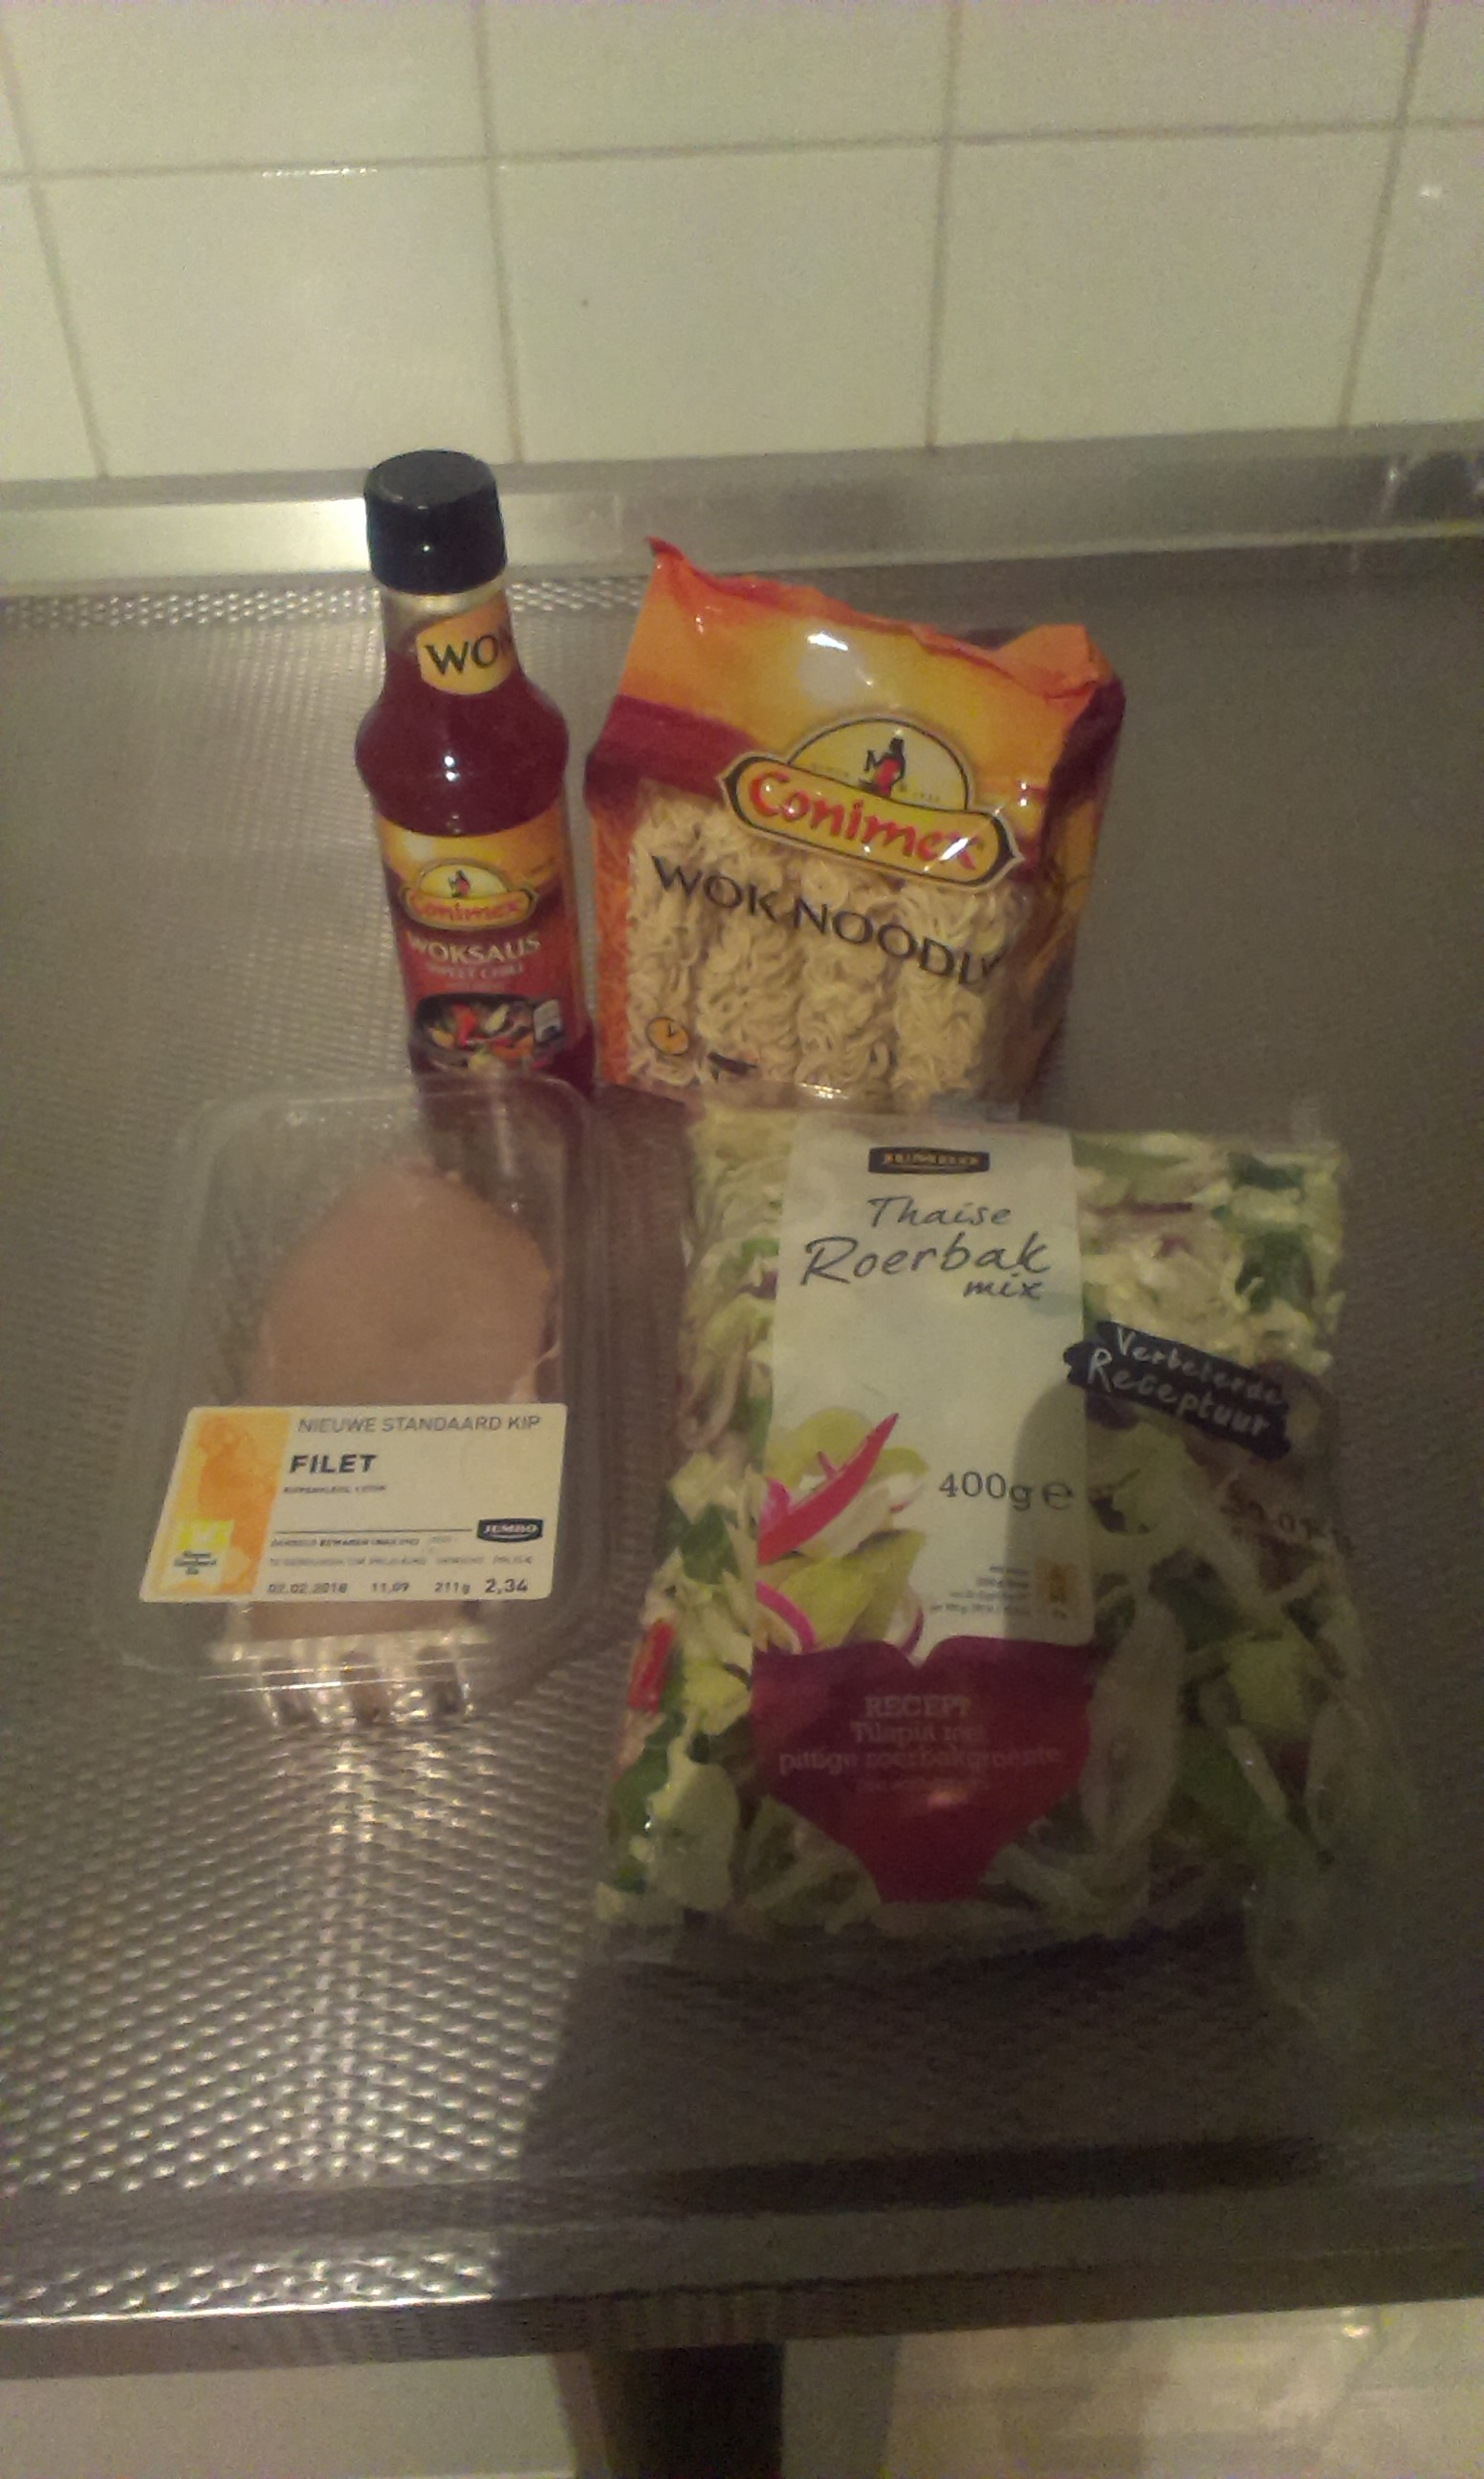
\includegraphics[width=35mm,scale=0.07]{Images/noodles_ingredients.jpg}
\end{minipage}
\end{figure}


\section*{Method}

\begin{figure}[h]

\begin{minipage}{0.5\textwidth}
Bake the chicken in a baking pan for a couple of minutes untill the chicken is nice light brown. In the meantime, put the noodles in boiling water for a couple of minutes in a seperate pan. \\
\\
Add the vegetables to the chicken and let it bake for another $5$-$10$ minutes (depending on your own preference). Drain the noodles and them together with the sauce. \\
\\
Mix everyhting and... that's it!

\end{minipage}
\begin{minipage}{0.4\textwidth}
	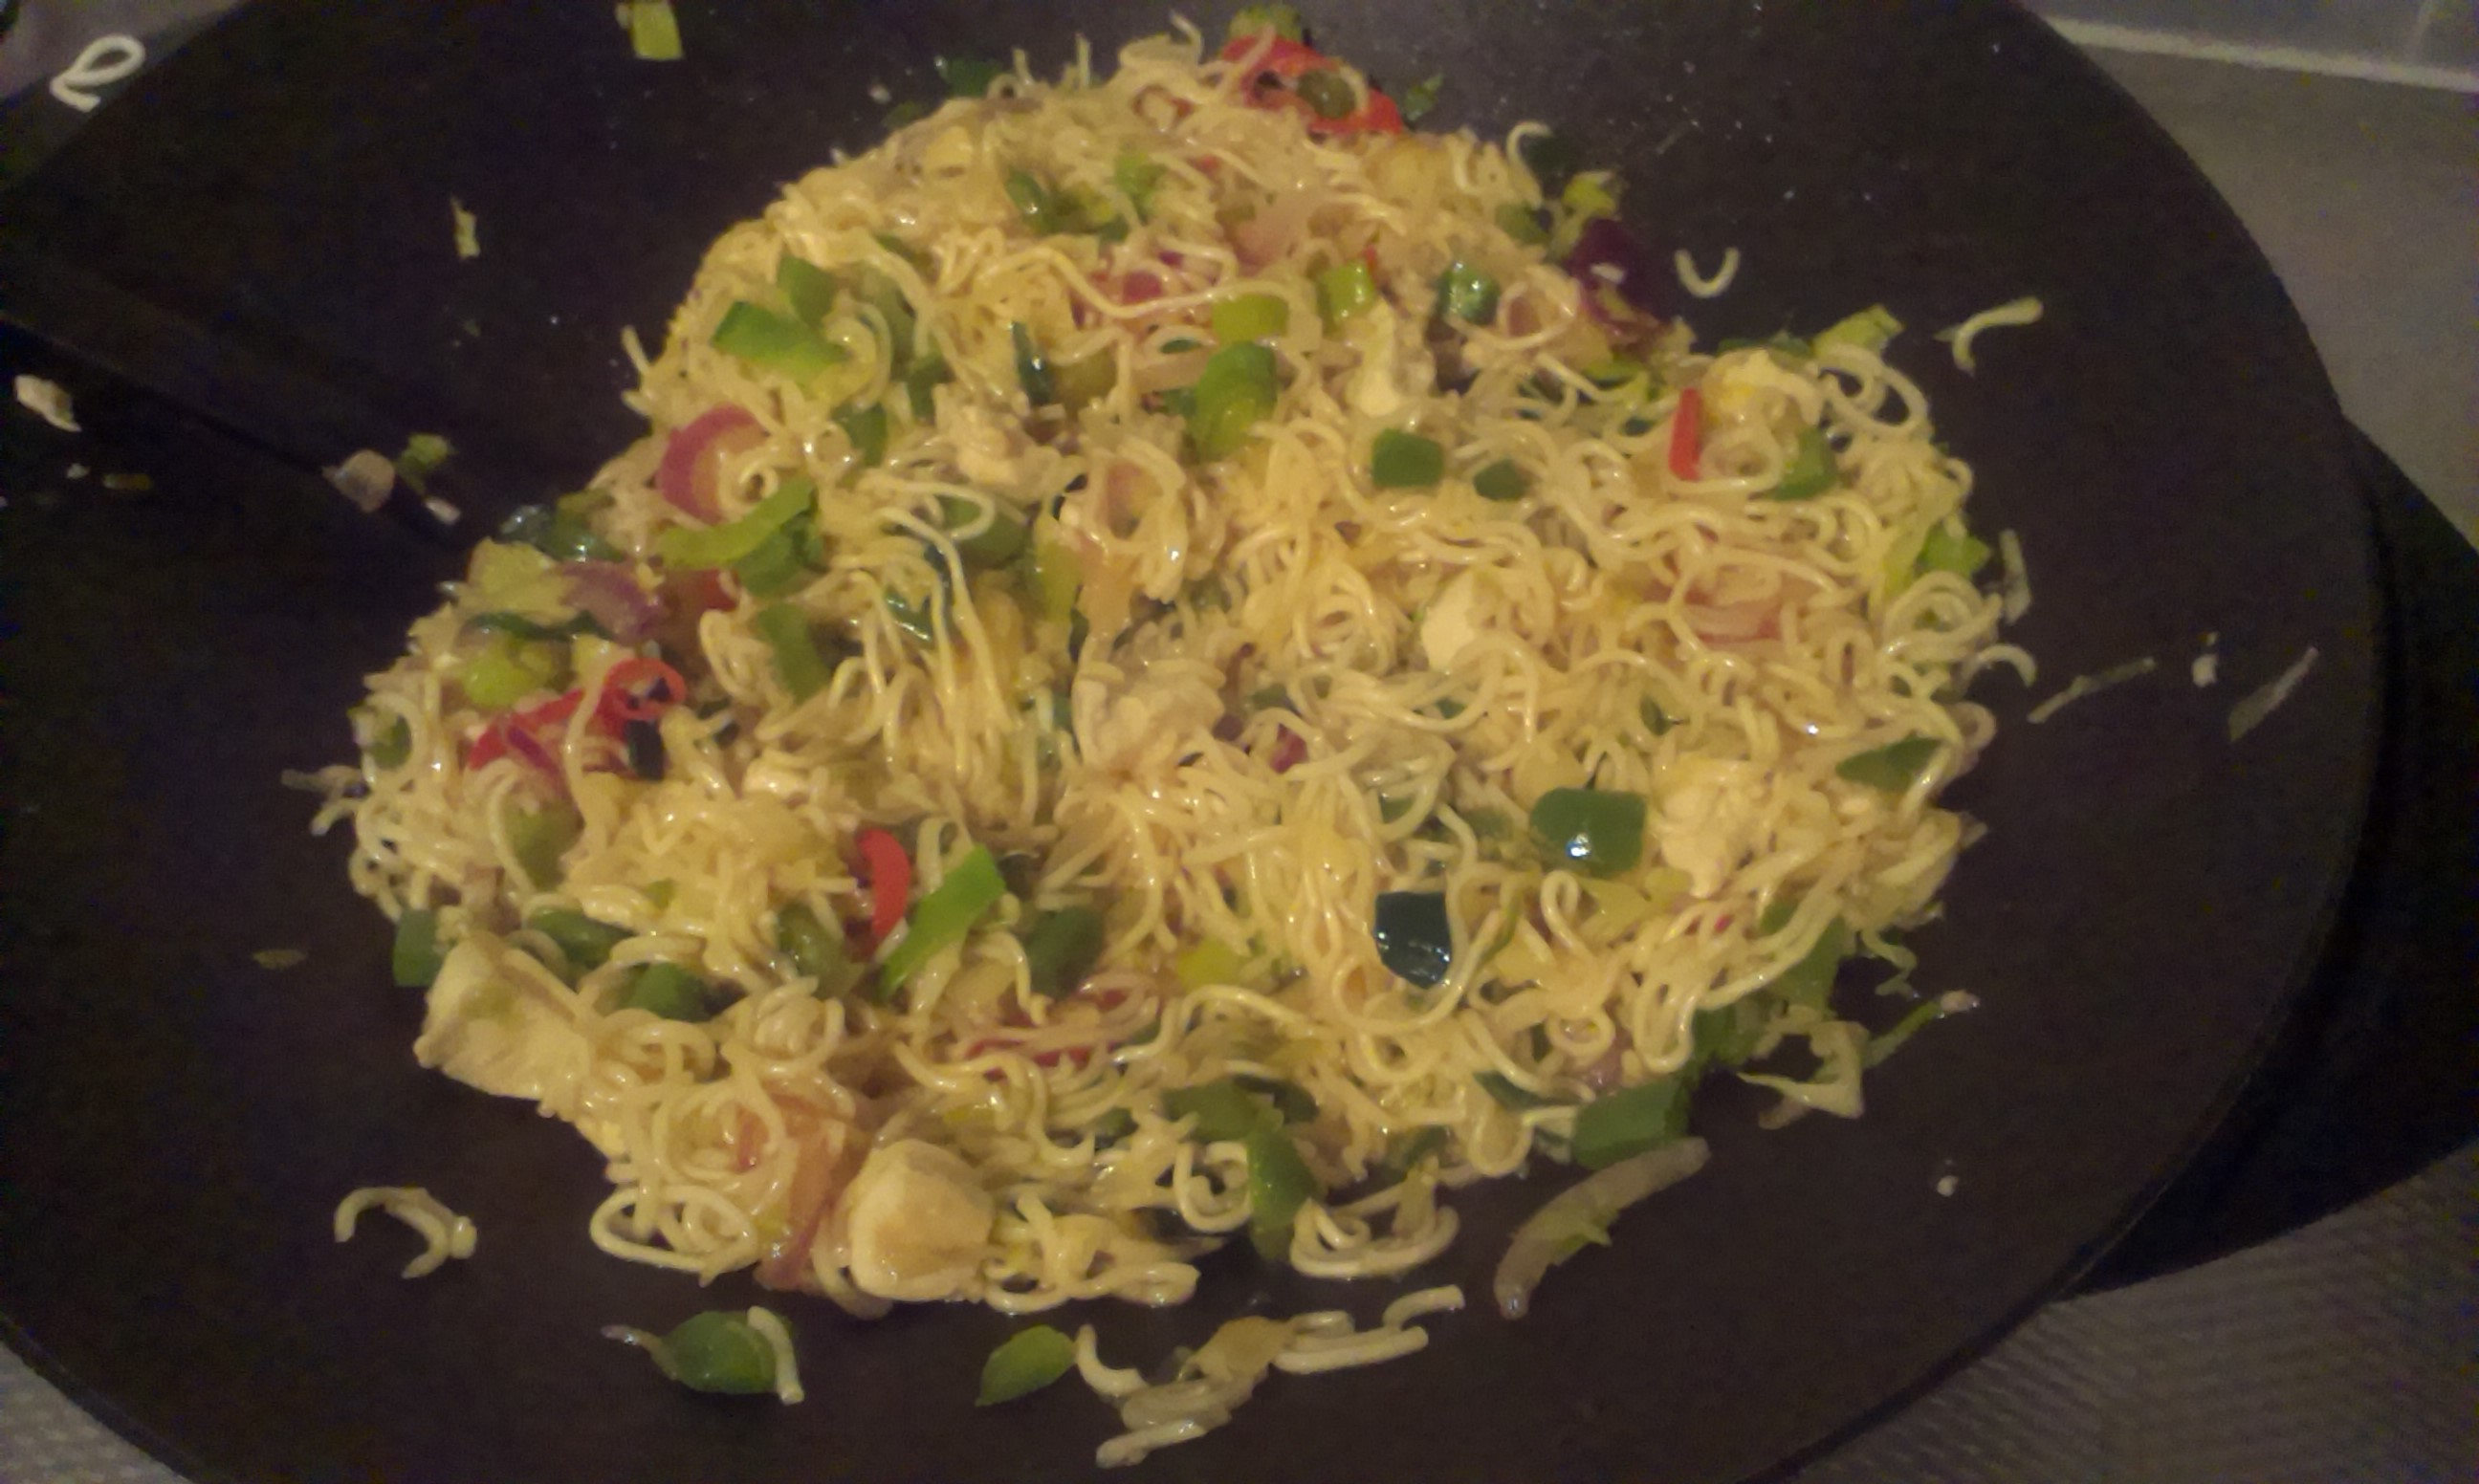
\includegraphics[scale=0.065]{Images/noodles.jpg}
\end{minipage}
\end{figure}

\newpage

\chapter{Ravioli with mushrooms and lentils}

\section*{Ingredients}
\begin{figure}[h]

\begin{minipage}{0.65\textwidth}
\begin{itemize}
\item Ravioli ($250$ gr.)
\item Hak bolognese `schotel' ($500$ gr.)
\item Mushrooms ($400$ gr.)
\item Parmezan cheese ($50$ gr.)
\end{itemize}
\end{minipage}
\begin{minipage}{0.3\textwidth}
	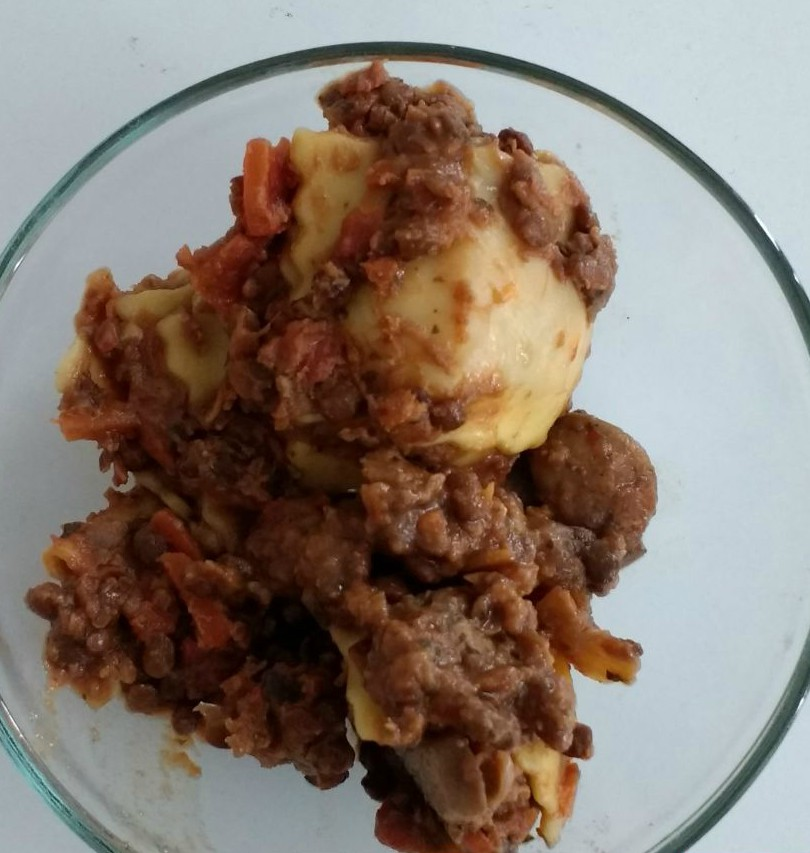
\includegraphics[scale=0.17]{Images/ravioliend.jpg}
\end{minipage}
\end{figure}


\section*{Method}

\begin{figure}[h]

\begin{minipage}{0.6\textwidth}
Cut the mushrooms and bake them in a baking pan for five minutes untill they are nice brown. In the meantime, put the ravioli in boiling water for approximately two minutes in a seperate pan.  \\
\\
Add the bolgenese `schotel' and let it bake for another five minutes on a medium heat. Add the ravioli and mix everything. Finish the dish with some nice cheese on top!

\end{minipage}
\begin{minipage}{0.35\textwidth}
	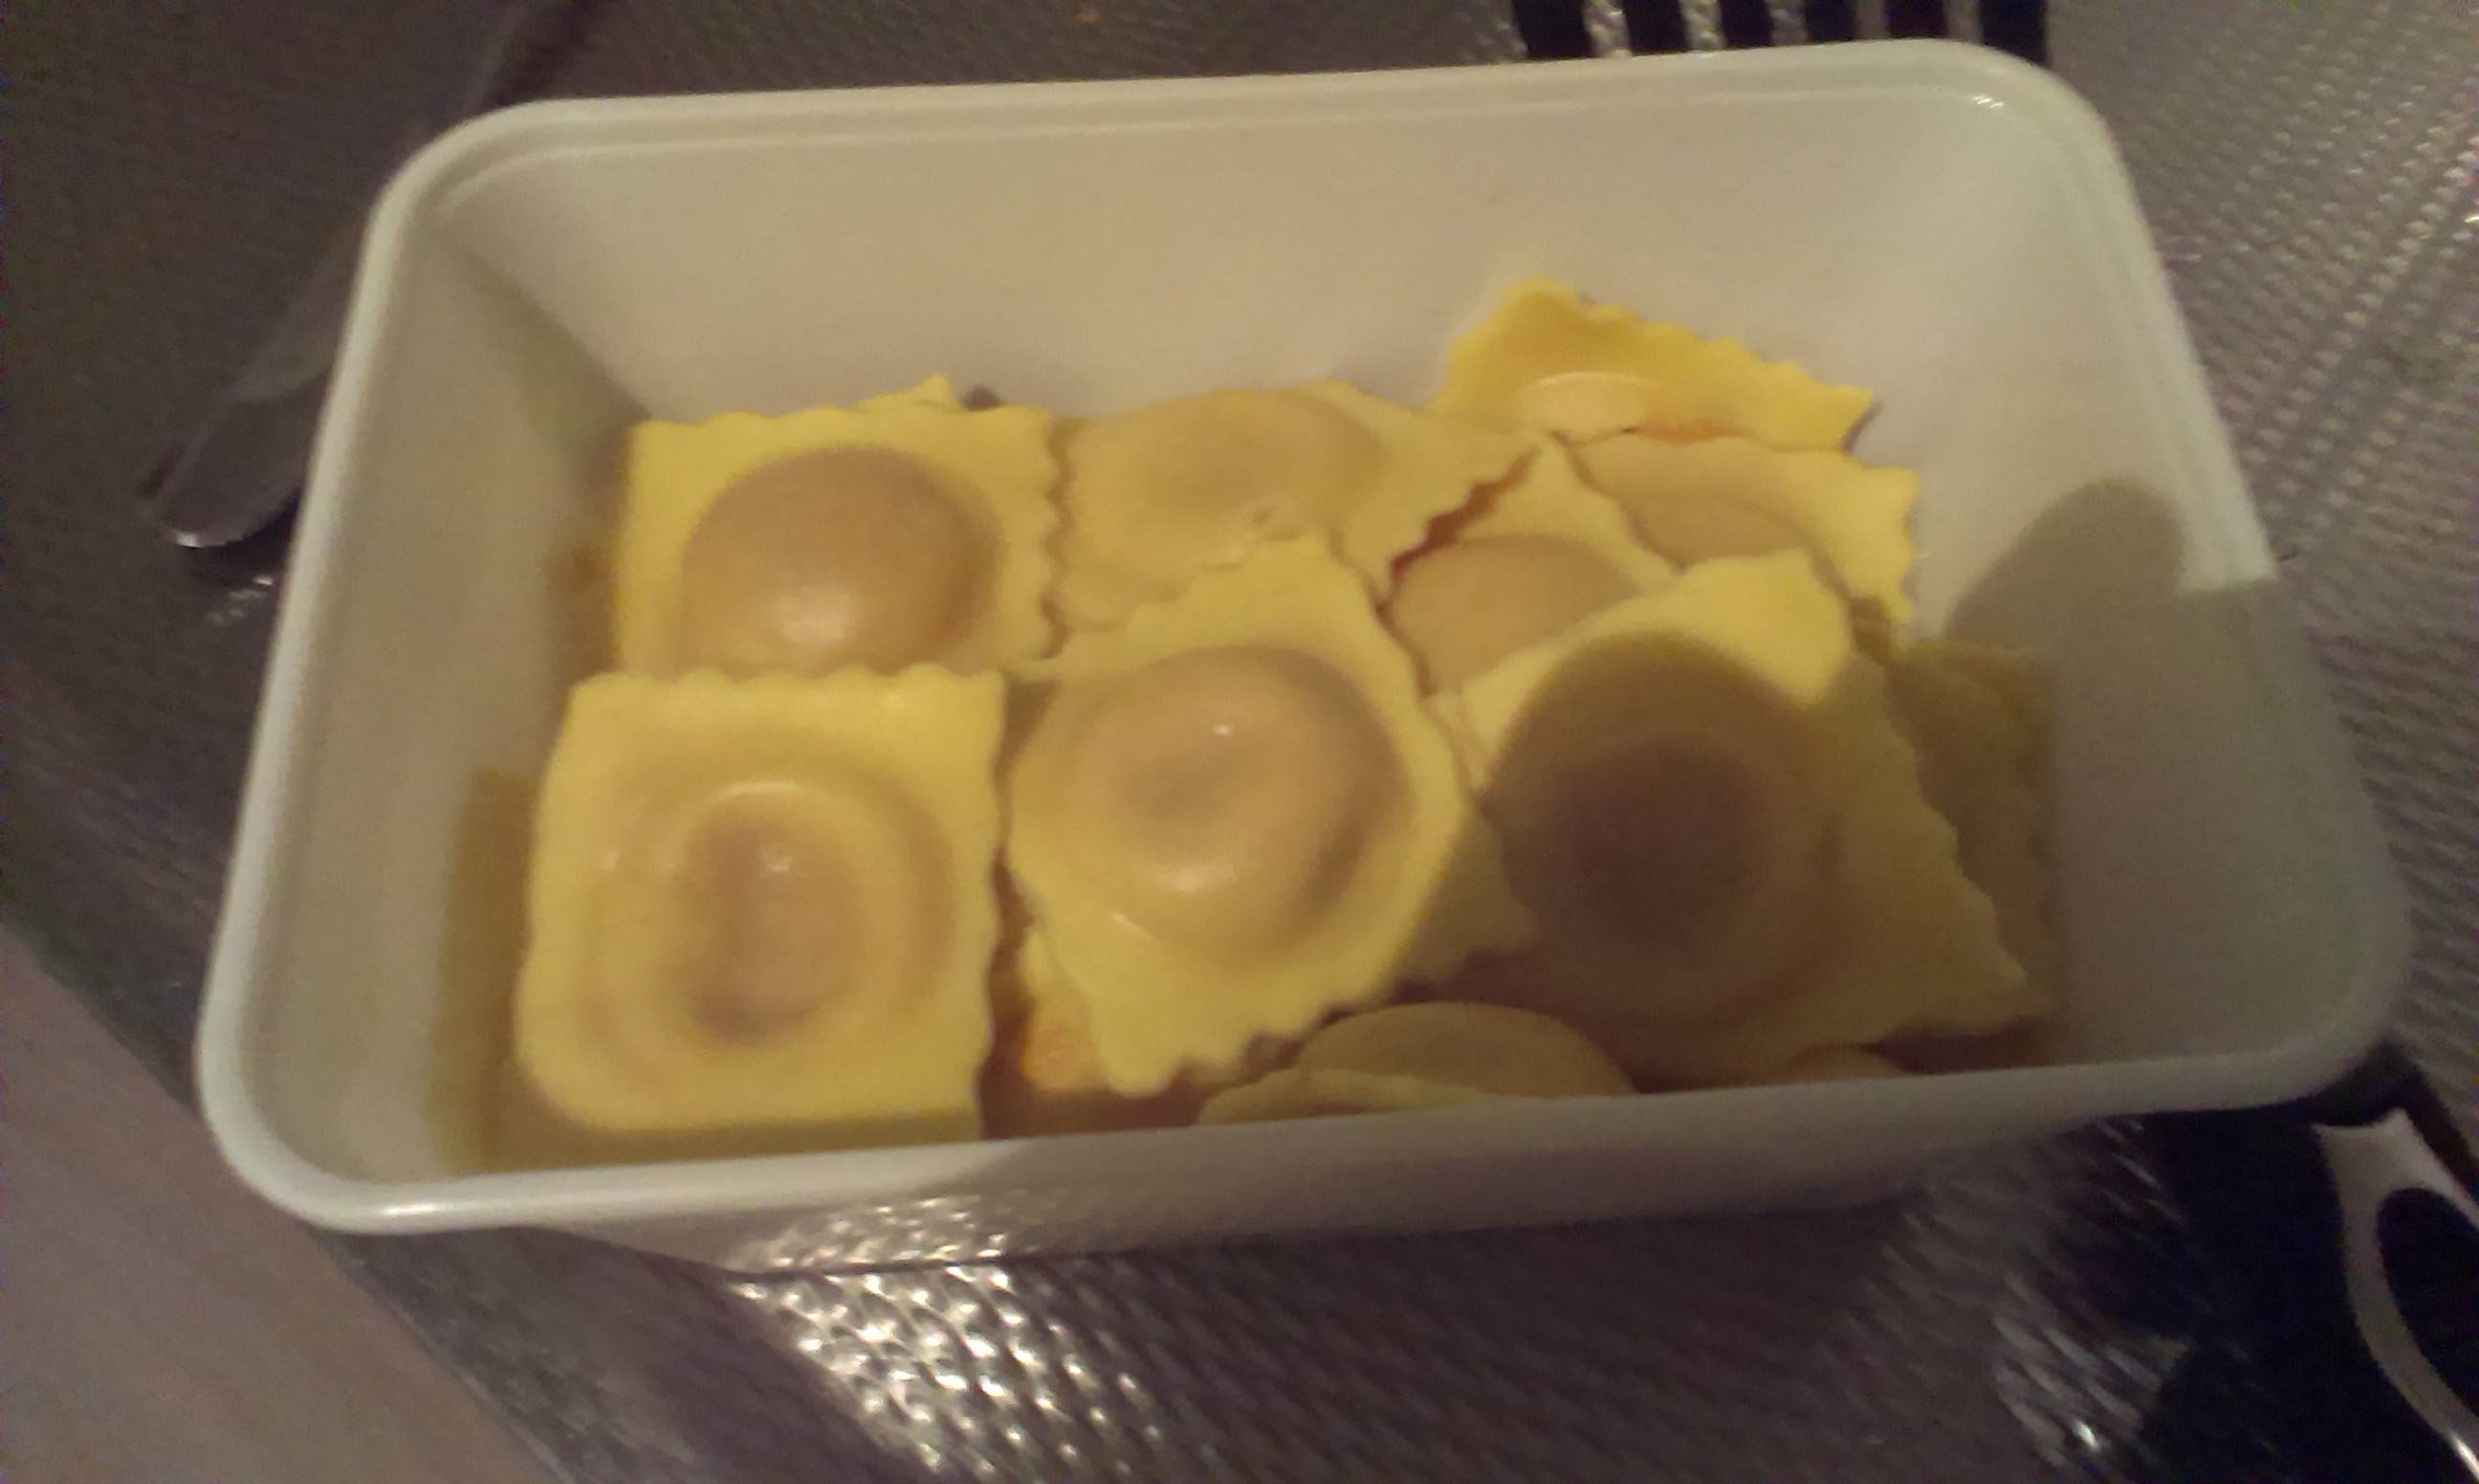
\includegraphics[scale=0.065]{Images/ravioli.jpg}
	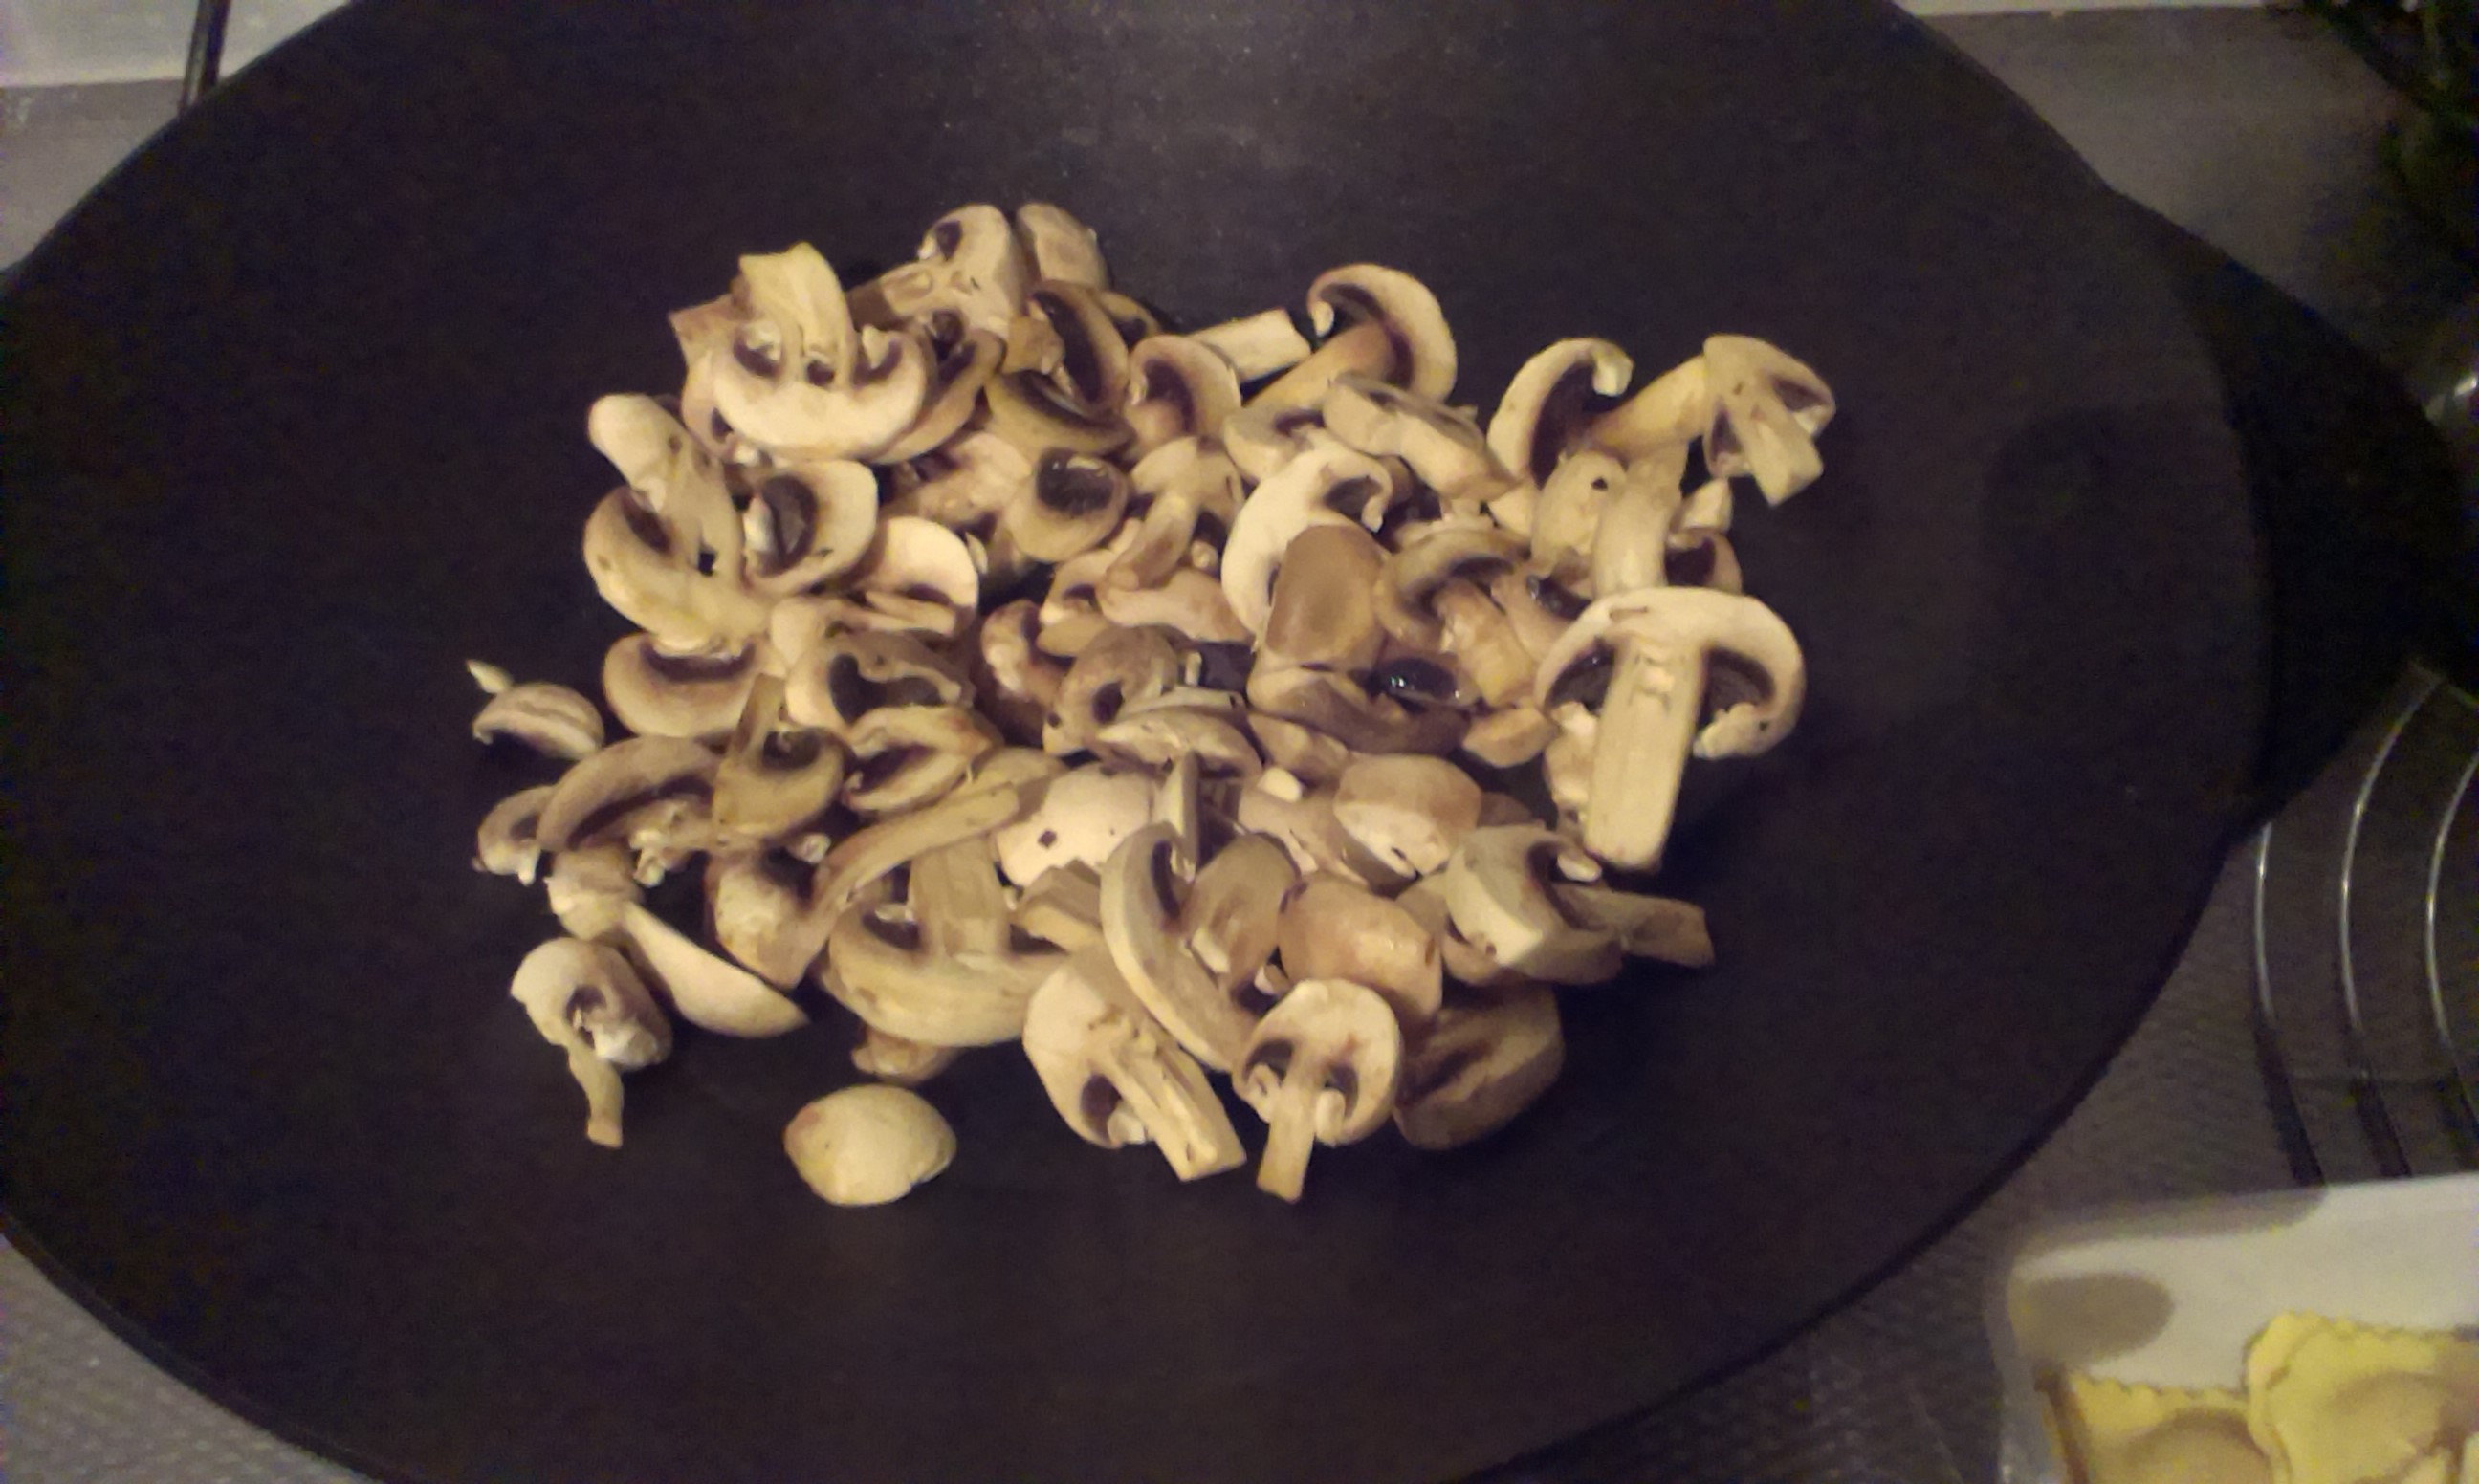
\includegraphics[scale=0.065]{Images/mushroom.jpg}
\end{minipage}
\end{figure}



\end{document}